\chapter{Разработка системы}
%3. Материалы главы 3 пояснительнои записки. Материалы могут быть представлены не в полном объеме. Обязательным является наличие пункта Технологические особенности реализации системы.

\section{Технологические особенности реализации системы}

\subsection{Выбор программных средств}

В качестве основного языка программирования выбран Python. Python очень популярен среди ученых и, в частности, среди специалистов по компьютерному зрению.

Некоторые скрипты для установки и обновления ПО будут написаны на языке Bash, так как это основной язык, используемый для автоматизации задач в среде UNIX.

\begin{figure}[h]
  \centering
  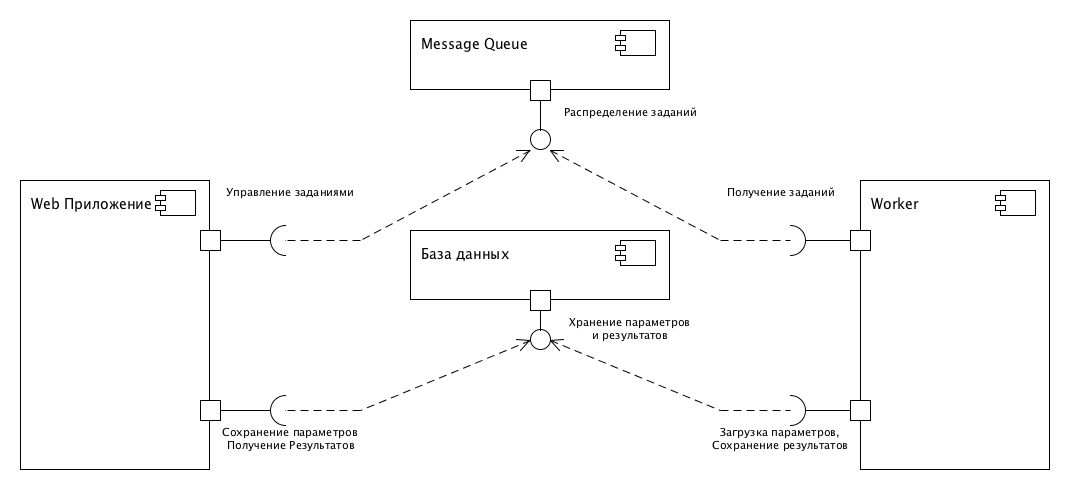
\includegraphics[width=1\textwidth]{assets/components-1.png}
  \caption{Компоненты системы}
  \label{fig:fig01}
\end{figure}



\section{Пользовательский интерфейс}

\subsection{Интерфейс системы развертки}

Поскольку работать с системой развертки будут опытные пользователи, в качестве интерфейса для этой программы предлагается интерфейс командной строки.

\subsection{Интерфейс системы управления кластером }

Пользовательский интерфейс системы управления кластером было решено сделать с применением web-технологий: HTML5, Java Script и CSS Использование web-технологий позволит быстро и просто создавать необходимые интерфейсы, а также делает решение более привычным для неподготовленных пользователей. На стороне сервера используется web-фреймворк Django - популярное решение в среде программистов на Python. Современный уровень развития web-технологий позволяет создавать полноценные кросс-платформенные интерфейсы.

Основные интерфейсы представлены ниже:
\begin{figure}[h]
  \centering
  % \fbox{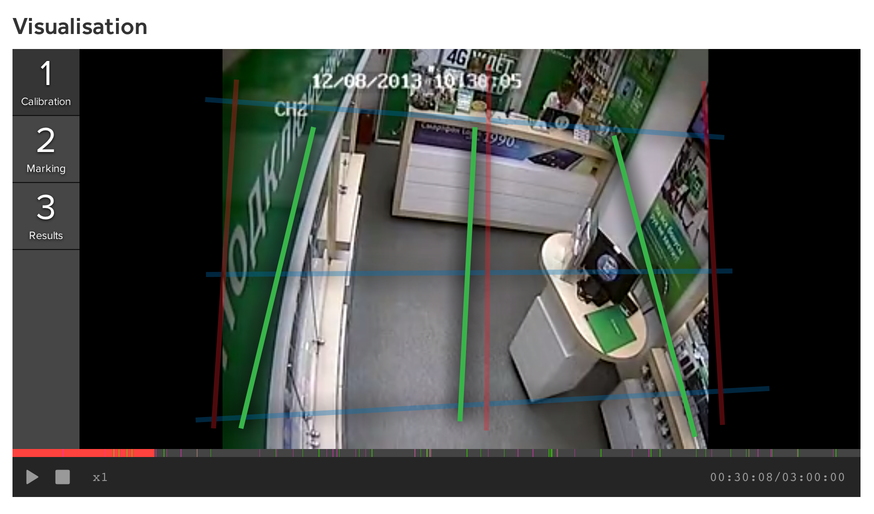
\includegraphics[width=0.8\textwidth]{assets/interface-1.png}}
  \fbox{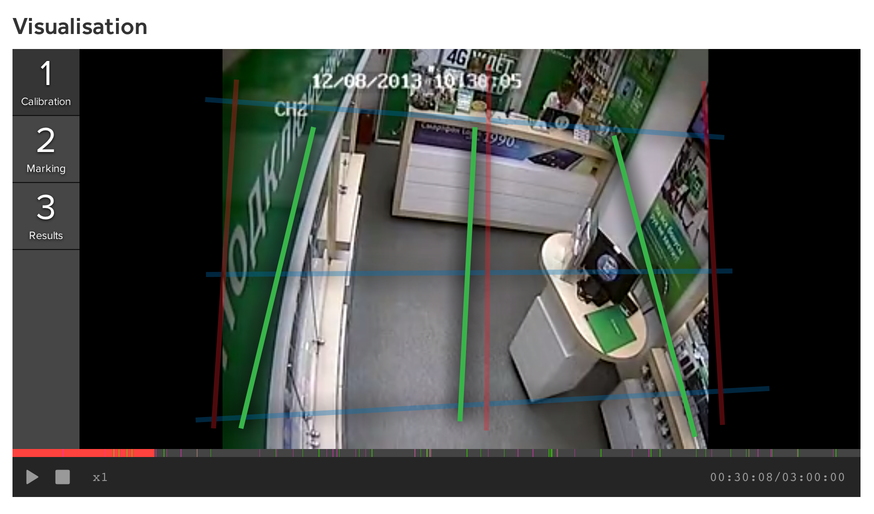
\includegraphics[width=0.8\textwidth]{assets/interface-1.png}}
  \caption{Интерфейс настройки пространственных параметров}
  \label{fig:fig01}
\end{figure}

На рисунке \ref{fig:fig01} показан интерфейс настройки пространственных параметров. Пользователю предлагается нарисовать по 3 линии в 3-х проекциях. Эта информация затем будет использована алгоритмом слежения для корректирования изображения.

\begin{figure}[h]
  \centering
  % \fbox{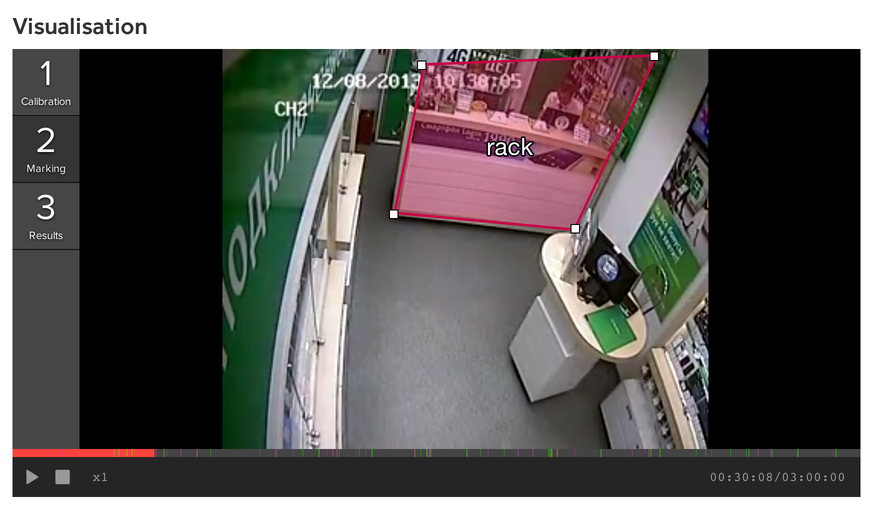
\includegraphics[width=0.8\textwidth]{assets/interface-2.png}}
  \fbox{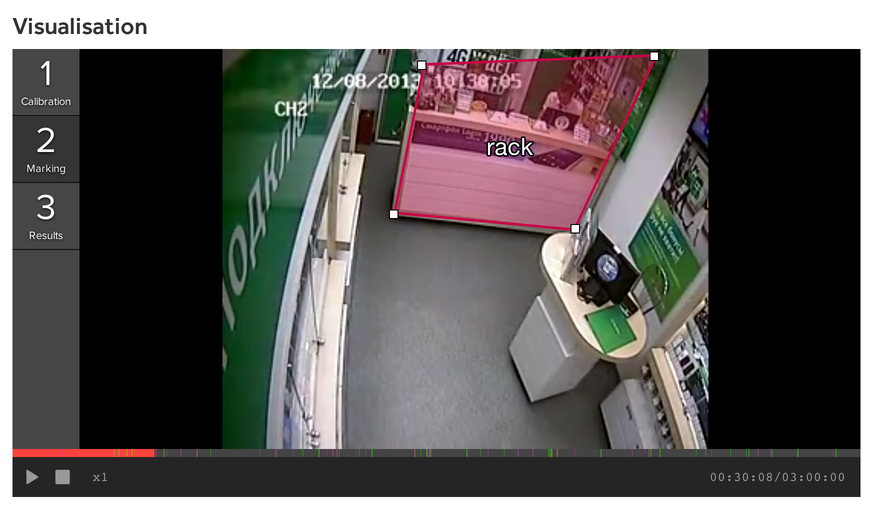
\includegraphics[width=0.8\textwidth]{assets/interface-2.png}}
  \caption{Интерфейс разметки на зоны}
  \label{fig:fig02}
\end{figure}

Для определения пересечения тракторий людей с некоторыми зонами, эти зоны необходимо сначала определить. Для этого пользователю предлагается нарисовать эти зоны на изображении (рис. \ref{fig:fig02}).

\begin{figure}[h]
  \centering
  % \fbox{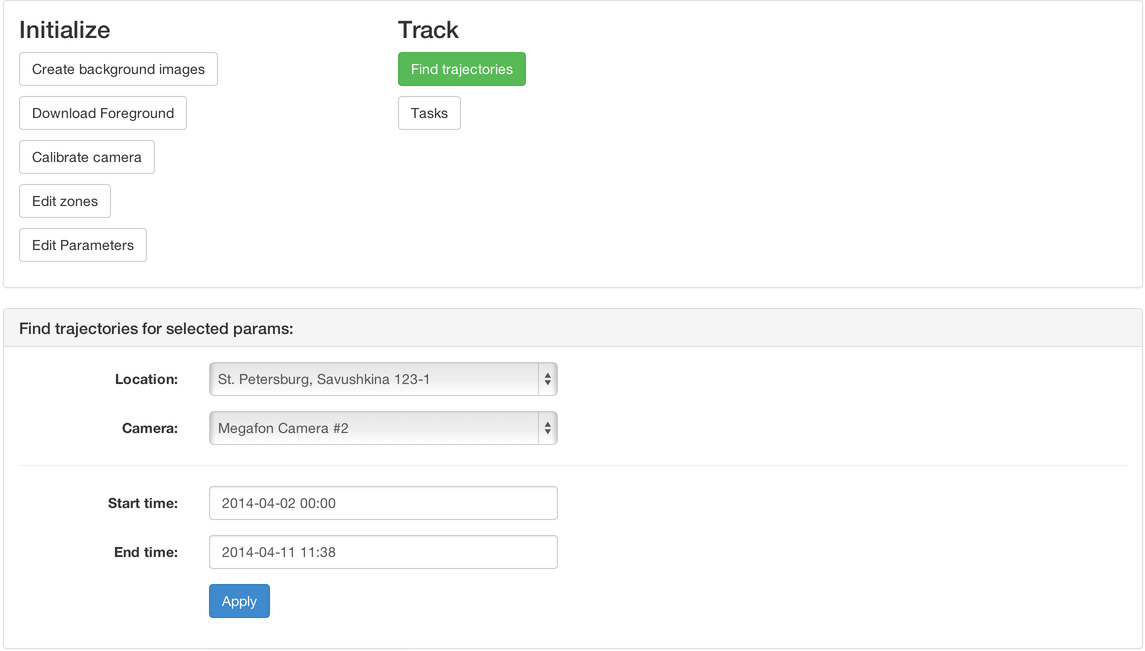
\includegraphics[width=0.8\textwidth]{assets/interface-0.png}}
  \fbox{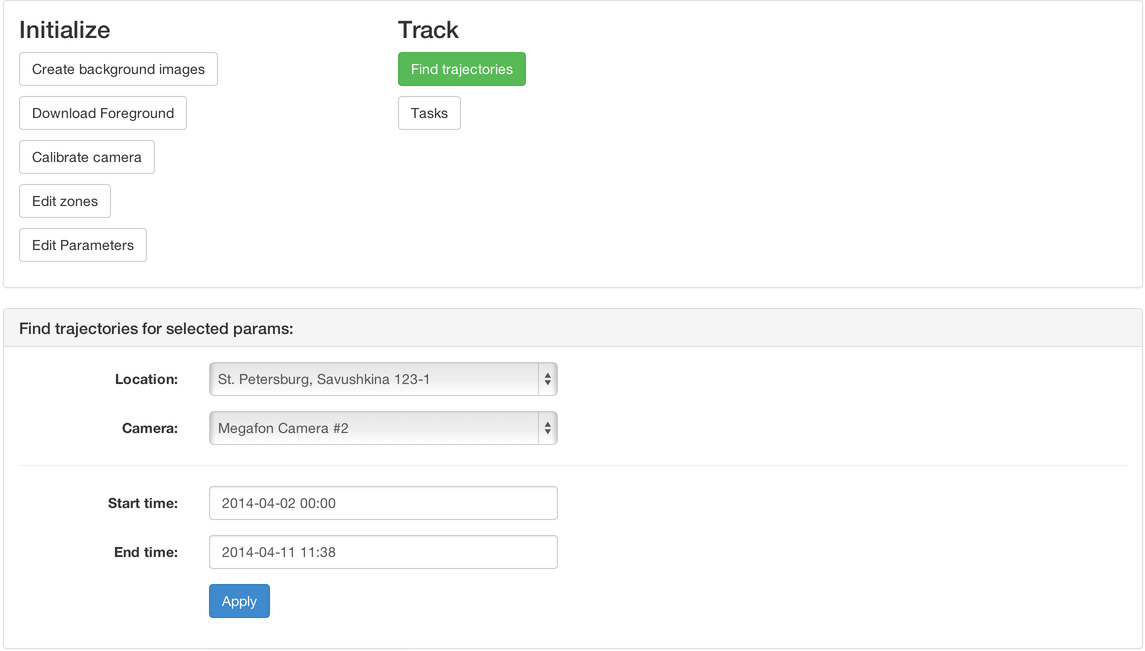
\includegraphics[width=0.8\textwidth]{assets/interface-0.png}}
  \caption{Интерфейс управления заданиями}
  \label{fig:fig03}
\end{figure}

После того, как предварительный этап закончен, можно запускать алгоритм слежения. Пользователю предлагается выбрать нужную камеру и временной период, видео в котором нужно обработать (рис. \ref{fig:fig03}).

\begin{figure}[h]
  \centering
  % \fbox{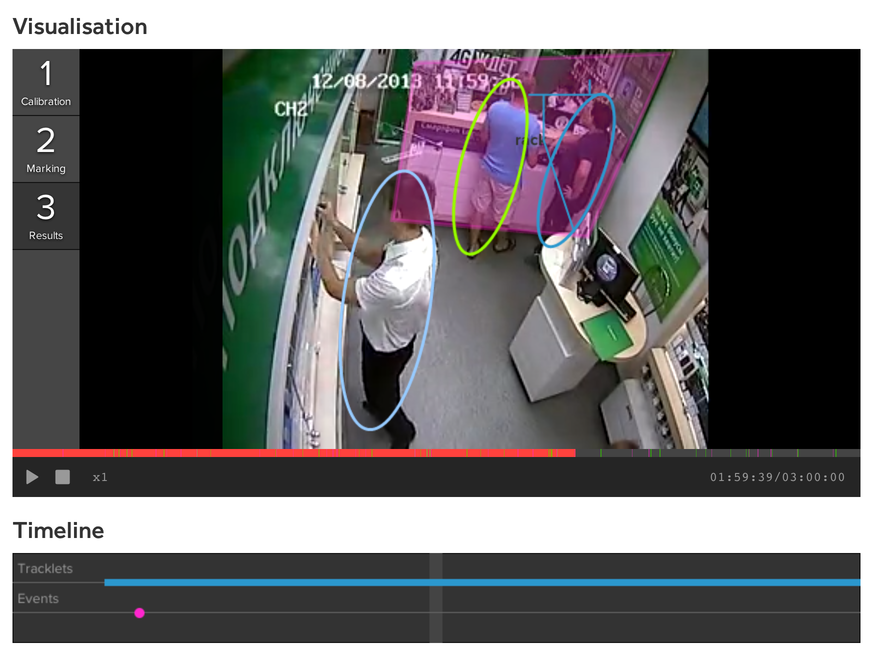
\includegraphics[width=0.8\textwidth]{assets/interface-3.png}}
  \fbox{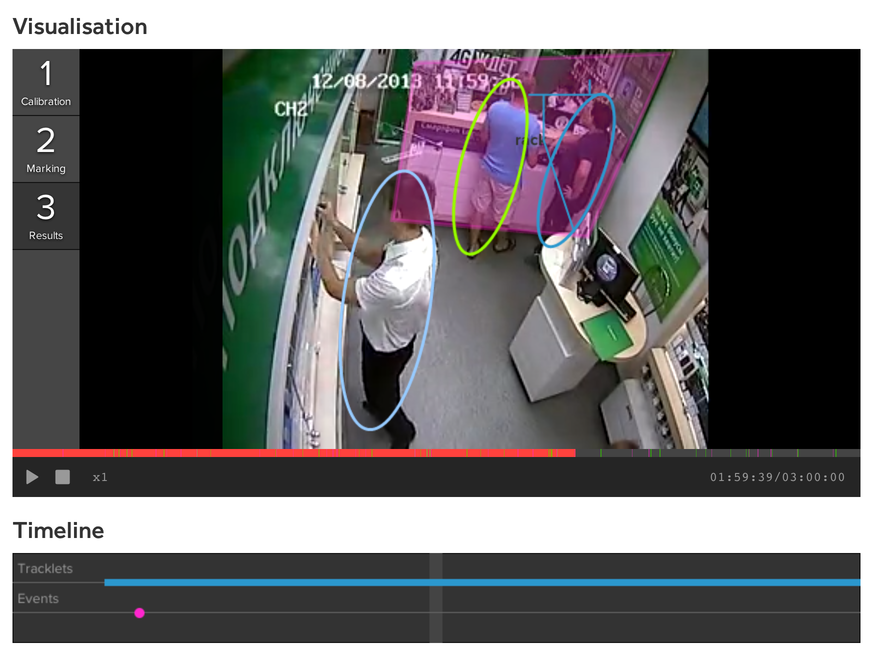
\includegraphics[width=0.8\textwidth]{assets/interface-3.png}}
  \caption{Интерфейс просмотра результатов}
  \label{fig:fig04}
\end{figure}

После того, как алгоритм закончил работу можно посмотреть результаты, для этого пользователю предлагается просмотр видео и отмеченными на нем ключевыми моментами, такими как входы и выходы из зон (рис. \ref{fig:fig04}).



%\section{План тестирования}
